\documentclass[12pt]{article}

\usepackage[utf8x]{inputenc} % Включаем поддержку UTF8  
\usepackage[russian]{babel}  % Включаем пакет для поддержки русского языка  
\usepackage{hyperref}        % Для гиперссылок

% Математика
\usepackage{amsmath}         % В т.ч. для матриц
\usepackage{amssymb}

% Прога
\usepackage{etoolbox}
\usepackage{listings}

% Цвета
\usepackage{xcolor}

% Картинки
\usepackage{graphicx}
\graphicspath{ {./images/} }

\newtheorem{property}{Свойство}
\newtheorem{consequence}{Следствие}[property]

\newcommand{\qedsymbol}{\rule{2mm}{2mm}}

\begin{document}

\thispagestyle{empty}
\begin{center}
\textbf{ПРАВИТЕЛЬСТВО РОССИЙСКОЙ ФЕДЕРАЦИИ}

\vspace{5ex}
	
\textbf{Федеральное государственное автономное образовательное учреждение \\ высшего образования \\ <<Национальный исследовательский университет \\ <<Высшая школа экономики>>}
\end{center}
\vspace{5ex}

\begin{center}
    Московский институт электроники и математики им. А.Н. Тихонова  
    
    \vspace{5ex}
    
    Департамент прикладной математики
    
    \vspace{10ex}
    \textbf{Отчёт \\ по лабораторной работе №4 \\ по курсу <<Алгоритмизация и программирование>>}
	\vspace{7ex}

\end{center}

\begin{center} 
\begin{tabular}{| p{0.3\linewidth}| p{0.3\linewidth}| p{0.3\linewidth}|}
 \hline	
ФИО студента & Номер группы & Дата \\  \hline
 & & \\  
Вязов Глеб \newline Дмитриевич & БПМ-231 & 18.11.2023\\  
 & & \\  \hline		
\end{tabular}
\end{center}

\begin{center}
	\vspace{3ex}
	
	\vfill
   
   \normalsize
    
	\textbf{Москва, 2023}
\end{center}

\newpage

%---------------------------------------------------------------------------------

\section*{Задание (вариант №7)}
Числовой массив B (тип массива указан в формулировке второго задания) содержит k элементов. Элементы массива и пороговые
значения X, Y вводятся с клавиатуры. Написать подпрограммы создания массива и вывода его на экран. В первом задании
требуется написать функцию нахождения соответствующего варианту максимального/минимального значения, а во втором –
среднего арифметического указанных в условии элементов ("между" понимать строго – не включая найденные позиции). 

Оба задания реализовать в одной программе.
\begin{enumerate}
\item $min(b_{1}, ..., b_{k})$ для $b_{i}>0$
\item Среднее арифметическое элементов, расположенных до последнего максимального элемента. Массив вещественный
\end{enumerate}


\newpage

%---------------------------------------------------------------------------------

\section*{Решение}\addcontentsline{toc}{section}{Решение}

\lstset{ %
texcl=true,%
language=C,                 % выбор языка для подсветки
basicstyle=\small\sffamily, % размер и начертание шрифта для подсветки кода
numbers=left,               % где поставить нумерацию строк (слева\справа)
numberstyle=\tiny,           % размер шрифта для номеров строк
stepnumber=1,                   % размер шага между двумя номерами строк
numbersep=5pt,                % как далеко отстоят номера строк от подсвечиваемого кода
backgroundcolor=\color{white}, % цвет фона подсветки - используем \usepackage{color}
showspaces=false,            % показывать или нет пробелы специальными отступами
showstringspaces=false,      % показывать или нет пробелы в строках
showtabs=false,             % показывать или нет табуляцию в строках
frame=single,              % рисовать рамку вокруг кода
tabsize=3,                 % размер табуляции по умолчанию равен 2 пробелам
captionpos=t,              % позиция заголовка вверху [t] или внизу [b] 
breaklines=true,           % автоматически переносить строки (да\нет)
breakatwhitespace=false, % переносить строки только если есть пробел
escapeinside={\%*}{*)},   % если нужно добавить комментарии в коде
inputencoding=utf8x,
extendedchars=\true
}

\begin{lstlisting}[label=string_code1,caption=C]
#include <stdio.h>
#include <math.h>
#include <stdlib.h>

unsigned int k;

// Поиск минимального элемента в вещественном массиве, длиной length, большего x
// Если такого элемента нет (то есть ai <= x для всех i), то возвращается NAN
double find_min_element(double *array, double x) {
    double min = array[0];
    for (int i=1; i < k; i++) {
        if (array[i] > x && (array[i] < min || min <= x)) {
            min = array[i];
        }
    }
    if (min <= x) {
        return NAN;
    }
    return min;
}

// Функция возвращает индекс последнего максимального элемента
int last_index_max_element(double *array) {
    double max = array[0];
    int index_max = 0;

    for (int i=0; i<k; i++) {
        if (max <= array[i]) {
            max = array[i];
            index_max = i;
        }
    }

    return index_max;
}

// Функция считает среднее арифметическое, расположенных до последнего максимального элемента
double mean(double *array) {
    double sum = 0;
    int current_len = last_index_max_element(array);
    if (current_len == 0) {
        return 0;
    }

    for (int i=0; i < current_len; i++) {
        sum += array[i];
    }

    return sum / current_len;
}

// Создание массива длиной length с вещественными элементами
void create_array(double *array) {
    for (int i=0; i<k; i++) {
        scanf("%lf", &array[i]);
    }
}

// Вывод массива длиной length с вещественными элементами
void print_array(double *array) {
    for (int i=0; i<k; i++) {
        printf("%10.4lf\t", array[i]);
    }
}

int main() {
    // Меняем кодировку на UTF-8, чтобы можно было писать на русском
    system("chcp 65001");
    // Ввод переменных. Дружественный интерфейс
    printf("Выполнил задание: Вязов Глеб. Группа: БПМ231\n");
    printf("Введите длину массива: ");
    scanf("%d", &k);

    // Выделение памяти для k элементов, размерности sizeof(double)
    // И инициализируем всё нулями
    double *array = calloc(k, sizeof(double));

    // Если память не выделилась -- возвращаем ошибку
    if (array == NULL) {
        return 1;
    }

    create_array(array);
    printf("Вы создали массив: ");
    print_array(array);

    double min = find_min_element(array, 0);
    if (isnan(min)) {
        printf("\nМинимальный элемент, больший 0: такого нет :(");
    } else {
        printf("\nМинимальный элемент, больший 0: %10.4lf", min);
    }
    printf("\nСреднее арифметическое до последнего максимального элемента: %10.4lf", mean(array));

    // Освобождаем память
    free(array);

    return 0;
}
\end{lstlisting} 

\newpage

%---------------------------------------------------------------------------------

\section*{Тестирование}

\begin{enumerate}

\item \textbf{Тест №1.} 

\textit{Ввод:} 3, -1, -2, 100

\textit{Вывод:} 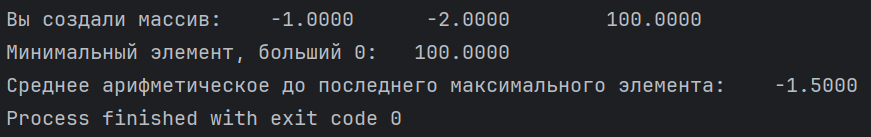
\includegraphics[width=0.9\textwidth]{img1}



\item \textbf{Тест №2.}

\textit{Ввод:} 1, 1

\textit{Вывод:} 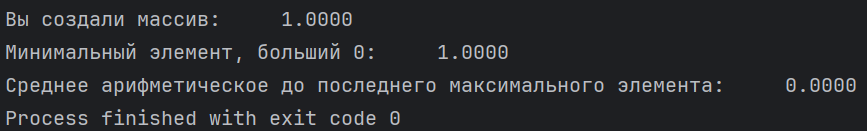
\includegraphics[width=0.9\textwidth]{img2}



\item \textbf{Тест №3.}

\textit{Ввод:} 4, 3.141516, 2.72459045, 5.78124678, -64.34

\textit{Вывод:} 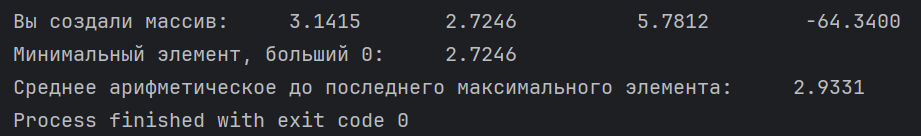
\includegraphics[width=0.9\textwidth]{img3}


\item \textbf{Тест №4.}

\textit{Ввод:} 3, -1, -2, -3

\textit{Вывод:} 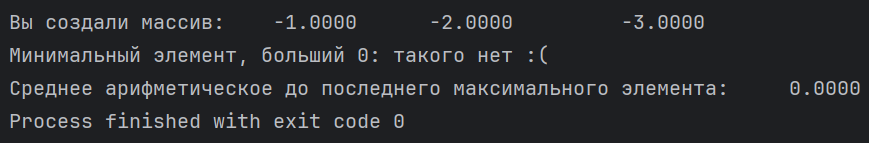
\includegraphics[width=0.9\textwidth]{img4}


\end{enumerate}


\end{document}
